\documentclass[../../../../main.tex]{subfiles}
\begin{document}

\begin{flushright}
\footnotesize\textit{【自動文字起こし・要確認】}
\end{flushright}

{\bf [解]}
\textbf{(1)} まず，面積が最大となる$\triangle PQR$は3頂点を正八角形の頂点としてよいことを示す．$Q,R$を固定すると，$\triangle PQR$の面積は$\frac12|QR|\cdot d(P,\text{直線}\,QR)$であり，$P$がある辺（線分）上を動くとき$d(P,\text{直線}\,QR)$は$P$の位置の1次式（アフィン関数）だから，最大値はその辺の端点（正八角形の頂点）のいずれかで実現する（辺が直線$QR$と平行なときは辺上で一定値をとり，端点でも同じ値になる）．よって$P$を頂点としてよく，$Q,R$についても同様だから，3頂点はすべて正八角形の頂点としてよい．

正八角形（1辺の長さ1）の外接円の半径を$R_0$とすると，$1=2R_0\sin\frac\pi8$より
\begin{align*}
R_0^2=\frac1{4\sin^2\frac\pi8}=\frac1{2\bigl(1-\cos\frac\pi4\bigr)}=\frac{2+\sqrt2}2.
\end{align*}
3頂点を選ぶとき，隣接する頂点間の辺の本数を$p,q,r$（$p+q+r=8$，$p,q,r\ge1$）とすると，中心角はそれぞれ$\frac{p\pi}4,\frac{q\pi}4,\frac{r\pi}4$であり，円に内接する三角形の面積公式より
\begin{align*}
\triangle=\frac12R_0^2\Bigl(\sin\frac{p\pi}4+\sin\frac{q\pi}4+\sin\frac{r\pi}4\Bigr).
\end{align*}
$(p,q,r)$の組合せ（並べ替えを除く）は$(1,1,6),(1,2,5),(1,3,4),(2,2,4),(2,3,3)$の5通りで，それぞれ
\begin{align*}
(1,1,6):&\ \sin\frac\pi4+\sin\frac\pi4+\sin\frac{3\pi}2=\sqrt2-1,\\
(1,2,5):&\ \sin\frac\pi4+\sin\frac\pi2+\sin\frac{5\pi}4=1,\\
(1,3,4):&\ \sin\frac\pi4+\sin\frac{3\pi}4+\sin\pi=\sqrt2,\\
(2,2,4):&\ \sin\frac\pi2+\sin\frac\pi2+\sin\pi=2,\\
(2,3,3):&\ \sin\frac\pi2+\sin\frac{3\pi}4+\sin\frac{3\pi}4=1+\sqrt2.
\end{align*}
最大は$(2,3,3)$型（例えば$\triangle A_2A_5A_7$）で，
\begin{align*}
\max S=\frac12\cdot\frac{2+\sqrt2}2\cdot(1+\sqrt2)=\frac{(2+\sqrt2)(1+\sqrt2)}4=\frac{4+3\sqrt2}4=1+\frac{3\sqrt2}4.
\end{align*}

\begin{figure}[htb]
\centering
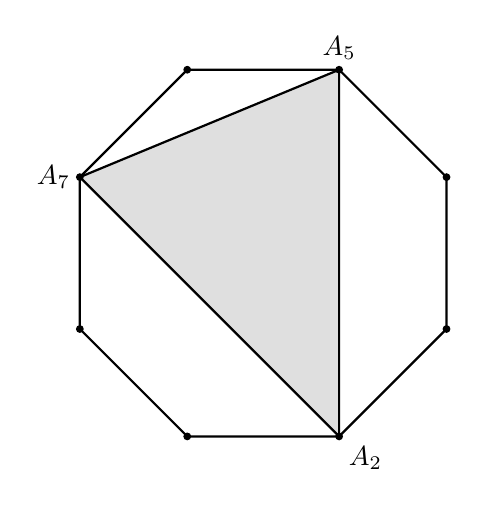
\begin{tikzpicture}[scale=1.4]
  \foreach \i/\ang in {1/-112.5,2/-67.5,3/-22.5,4/22.5,5/67.5,6/112.5,7/157.5,8/-157.5} {
    \coordinate (A\i) at (\ang:1.8);
  }
  \draw[thick] (A1)--(A2)--(A3)--(A4)--(A5)--(A6)--(A7)--(A8)--cycle;
  \fill[gray!25] (A2)--(A5)--(A7)--cycle;
  \draw[thick] (A2)--(A5)--(A7)--cycle;
  \foreach \i in {1,...,8}{\filldraw (A\i) circle(0.03);}
  \node[below right] at (A2) {$A_2$};
  \node[above] at (A5) {$A_5$};
  \node[left] at (A7) {$A_7$};
\end{tikzpicture}
\caption{(1)で面積が最大となる配置の一例：$\triangle A_2A_5A_7$（$(2,3,3)$型）}
\end{figure}

\textbf{(2)} 対称性より$Q=A_1$としてよい．正八角形の内角は$135^\circ$であり，$\angle PQR=90^\circ$なので，(1)と同様の議論（$P,R$を固定するときの端点最大性）から，$P,R$は$Q$に隣接する2辺（$A_1A_2$，$A_1A_8$）から最も離れた側の辺，具体的には辺$A_7A_8$と辺$A_3A_4$上にある場合に最大値の候補が現れる（他の配置はこれ以下になることが同様の議論で確かめられる）．

$A_1$を原点，$A_2=(1,0)$となるように座標を取ると，正八角形の頂点は
\begin{align*}
A_1=(0,0),\ A_2=(1,0),\ A_3=\Bigl(1+\tfrac{\sqrt2}2,\tfrac{\sqrt2}2\Bigr),\ A_4=\Bigl(1+\tfrac{\sqrt2}2,1+\tfrac{\sqrt2}2\Bigr),
\end{align*}
\begin{align*}
A_5=(1,1+\sqrt2),\ A_6=(0,1+\sqrt2),\ A_7=\Bigl(-\tfrac{\sqrt2}2,1+\tfrac{\sqrt2}2\Bigr),\ A_8=\Bigl(-\tfrac{\sqrt2}2,\tfrac{\sqrt2}2\Bigr).
\end{align*}
$P$は辺$A_7A_8$（$x=-\frac{\sqrt2}2$）上，$R$は辺$A_3A_4$（$x=1+\frac{\sqrt2}2$）上だから
\begin{align*}
P=\Bigl(-\frac{\sqrt2}2,a\Bigr),\quad R=\Bigl(1+\frac{\sqrt2}2,b\Bigr)\qquad\Bigl(\frac{\sqrt2}2\le a,b\le\frac{\sqrt2}2+1\Bigr).
\end{align*}

\begin{figure}[htb]
\centering
\begin{tikzpicture}[scale=1.4]
  \foreach \i/\ang in {1/-112.5,2/-67.5,3/-22.5,4/22.5,5/67.5,6/112.5,7/157.5,8/-157.5} {
    \coordinate (A\i) at (\ang:1.8);
  }
  \draw[thick] (A1)--(A2)--(A3)--(A4)--(A5)--(A6)--(A7)--(A8)--cycle;
  \coordinate (P) at ($(A7)!0.4!(A8)$);
  \coordinate (R) at ($(A3)!0.4!(A4)$);
  \fill[gray!25] (P)--(A1)--(R)--cycle;
  \draw[thick,blue] (P)--(A1)--(R);
  \filldraw (A1) circle(0.03) node[below]{$Q=A_1$};
  \filldraw (P) circle(0.03) node[left]{$P$};
  \filldraw (R) circle(0.03) node[right]{$R$};
\end{tikzpicture}
\caption{(2)の配置：$Q=A_1$固定，$P\in A_7A_8$，$R\in A_3A_4$，$\angle PQR=90^\circ$}
\end{figure}

$\angle PQR=90^\circ$は$\overrightarrow{QP}\cdot\overrightarrow{QR}=0$と同値：
\begin{align*}
\Bigl(-\frac{\sqrt2}2\Bigr)\Bigl(1+\frac{\sqrt2}2\Bigr)+ab=0\quad\therefore\ ab=\frac{\sqrt2}2\Bigl(1+\frac{\sqrt2}2\Bigr)=\frac{1+\sqrt2}2.\tag{①}
\end{align*}
$Q$が原点だから，三角形の面積公式$S=\frac12|x_Py_R-x_Ry_P|$より
\begin{align*}
S=\frac12\Bigl|\Bigl(-\frac{\sqrt2}2\Bigr)b-\Bigl(1+\frac{\sqrt2}2\Bigr)a\Bigr|
=\frac12\Bigl\{\Bigl(1+\frac{\sqrt2}2\Bigr)a+\frac{\sqrt2}2b\Bigr\}
\end{align*}
（$a,b>0$より絶対値ははずせる）．①より$b=\dfrac{1+\sqrt2}{2a}$を代入すると
\begin{align*}
S=\frac12\Bigl(1+\frac{\sqrt2}2\Bigr)a+\frac{\sqrt2}4\cdot\frac{1+\sqrt2}a
\end{align*}
は$a>0$で下に凸であり，停留点は$a=\dfrac{\sqrt2}2$（区間$\bigl[\frac{\sqrt2}2,1+\frac{\sqrt2}2\bigr]$の左端）にあるので，$S$はこの区間上単調増加．よって$a=1+\dfrac{\sqrt2}2$（右端，このとき①より$b=\dfrac{\sqrt2}2$）で最大となり，
\begin{align*}
\max S=\frac12\Bigl\{\Bigl(1+\frac{\sqrt2}2\Bigr)^2+\frac12\Bigr\}=\frac12\Bigl(\frac32+\sqrt2+\frac12\Bigr)=1+\frac{\sqrt2}2.
\end{align*}
（$Q$を他の頂点にとる配置や，例えば$R$を頂点$A_4$に固定する配置では最大値は$\frac{1+\sqrt2}2\ (<1+\frac{\sqrt2}2)$にとどまることが確かめられ，これより小さい．）よって
\begin{align*}
\max S=1+\frac{\sqrt2}2.
\end{align*}


\newpage

\end{document}
